\chapter{Distinct Oscillatory Subnetworks in the Zebra Finch Auditory System}

\section{Abstract}
To understand how an auditory system processes complex sounds, it is essential to understand how the temporal envelope of sounds, i.e. the time-varying amplitude, is encoded by neural activity. We studied the temporal envelope of Zebra finch vocalizations, and show that it exhibits modulations in the 0-30Hz range, similar to human speech. We then build linear filter models to predict 0-30Hz LFP activity from the temporal envelopes of vocalizations, achieving surprisingly high performance for electrodes near thalamorecipient areas of Zebra finch auditory cortex. We then show that there are two spatially-distinct subnetworks that oscillate at different frequency bands, one subnetwork that oscillates around 19Hz, and another subnetwork that oscillates at 14Hz. These two subnetworks are present in every anatomical region. Finally we show that we can improve predictive performance with recurrent neural network models.

\section{Introduction}

Many animals use vocalizations to bond with each other, declare territory, signify the presence of predators, to beg for food, and other essential functions that enable their survival as a species. Human beings arguably have the most sophisticated vocalizations, our acoustically and temporally complex speech, comprised of a highly variable sequence of harmonic stacks and explosive bursts. Songbirds also have a sophisticated vocal repertoire, are capable of learning vocalizations through mimicry, and have auditory systems with a comparable complexity to that of mammals \cite{Brainard2013}. The study of Avian auditory systems can lead to a better understanding of the auditory systems of their mammalian counterparts.

A fundamental component to both human speech and Avian vocalizations is the temporal envelope, which is low-passed and slowly changing ($<$ 30Hz). The temporal envelope of human speech, ranging in frequency to 2-20Hz, is well represented in human auditory cortex \cite{Aiken2008}. The temporal modulation spectrum of speech, which is the spectrum of frequencies present in the temporal envelope, was found to have consistent peaks at 2Hz and 5Hz across multiple languages \cite{Ding2016}. \cite{Singh2003} explored the joint spectro-temporal modulation spectra of Zebra finch song, and found temporal modulation frequencies to be necessarily low ($<$ 50Hz).

Modulations of the temporal envelope have been shown to influence neural activity in Zebra finch auditory cortex \cite{Nagel2006}. In the work the researchers identified neurons that adapted their temporal integration timescale to the overall temporal envelope magnitude, integrating over shorter timescales for louder stimuli. Linear filter models were used in \cite{Pasley2012} to decode the temporal envelope of speech from human auditory areas. Taken together, these separate tracts of research show that temporal envelopes of vocalizations are encoded by both Zebra finch and human auditory neurons.

For our study we focused on 5-30Hz activity of the multi-electrode local field potential (LFP), in Zebra finch auditory cortex. The local field potential is a complex mixture of membrane currents from both synapses and voltage-gated ion channels \cite{Buzsaki2012b}. There is evidence in mammals that the auditory LFP is comprised of a nested hierarchy of timescales \cite{Lakatos2005}. Temporal envelope modulations occur in the 0-30Hz frequency band, and neural activity has been shown to follow the temporal envelope, but it is unknown in Avian auditory systems whether there are other frequencies of oscillation in the 0-30Hz band that coexist with the encoding of the temporal envelope, originated from independent processes. Our work first explores the temporal modulation spectra of vocalizations across the repertoire of the Zebra finch. Then we explore the 5-30Hz LFP, using linear and nonlinear models to predict multi-electrode LFP from the stimulus amplitude envelope.

\section{Results}

\subsection{The Temporal Modulation Spectrum of Zebra Finch Vocalizations}

The temporal modulation spectrum for a set of vocalizations is the set of frequencies for which the amplitude envelope oscillates. Figure 1 shows the approach we used to quantify the modulation spectrum of different types of vocalizations used in the experiment. Figure 1a shows examples of several vocalizations and their amplitude envelopes. Sequences of distance calls and tets comprise a category of ``affiliative calls'', and were repeated up to three times over two seconds, with random inter-call intervals ranging from 200-500ms. Figure 1b shows the average temporal modulation spectrum for affiliative calls (purple), which exhibit most power in the 2-5Hz range. Song, an example shown in the middle row of Figure 1a, had many fast syllable transitions and the average temporal modulation spectrum exhibited a peak from 6-10Hz. Begging calls, a fast repeating vocalization emitted only by juveniles, also exhibited higher temporal modulation frequencies. Modulation-limited noise (ML-noise) is a sound generated by noise that is constrained to have the same spectral and temporal modulations as Zebra finch song \cite{Hsu2004b}. The bottom row shows an example of an ML-noise stimulus and its amplitude envelope. The temporal modulation spectrum of ML-noise has a large DC component but very little power in the 5-30Hz range.

\begin{figure}
    \caption{\textbf{Temporal Modulation Frequencies of Vocalizations} We computed the temporal envelopes of Zebra finch vocalizations and their power spectra. \textbf{(a)} Three examples of Zebra finch vocalizations, shown by their spectrograms, and their temporal envelopes, shown in black. The top row is a Tet, a prolific affiliative communication call. The middle plot is a Zebra finch song, which was comprised of many closely spaced syllables. The bottom plot is modulation-limited (ML) noise, which had a highly variable temporal envelope. \textbf{(b)} The average temporal modulation spectra (the power spectra computed from temporal envelopes) for several vocalization categories.}
    \centering
    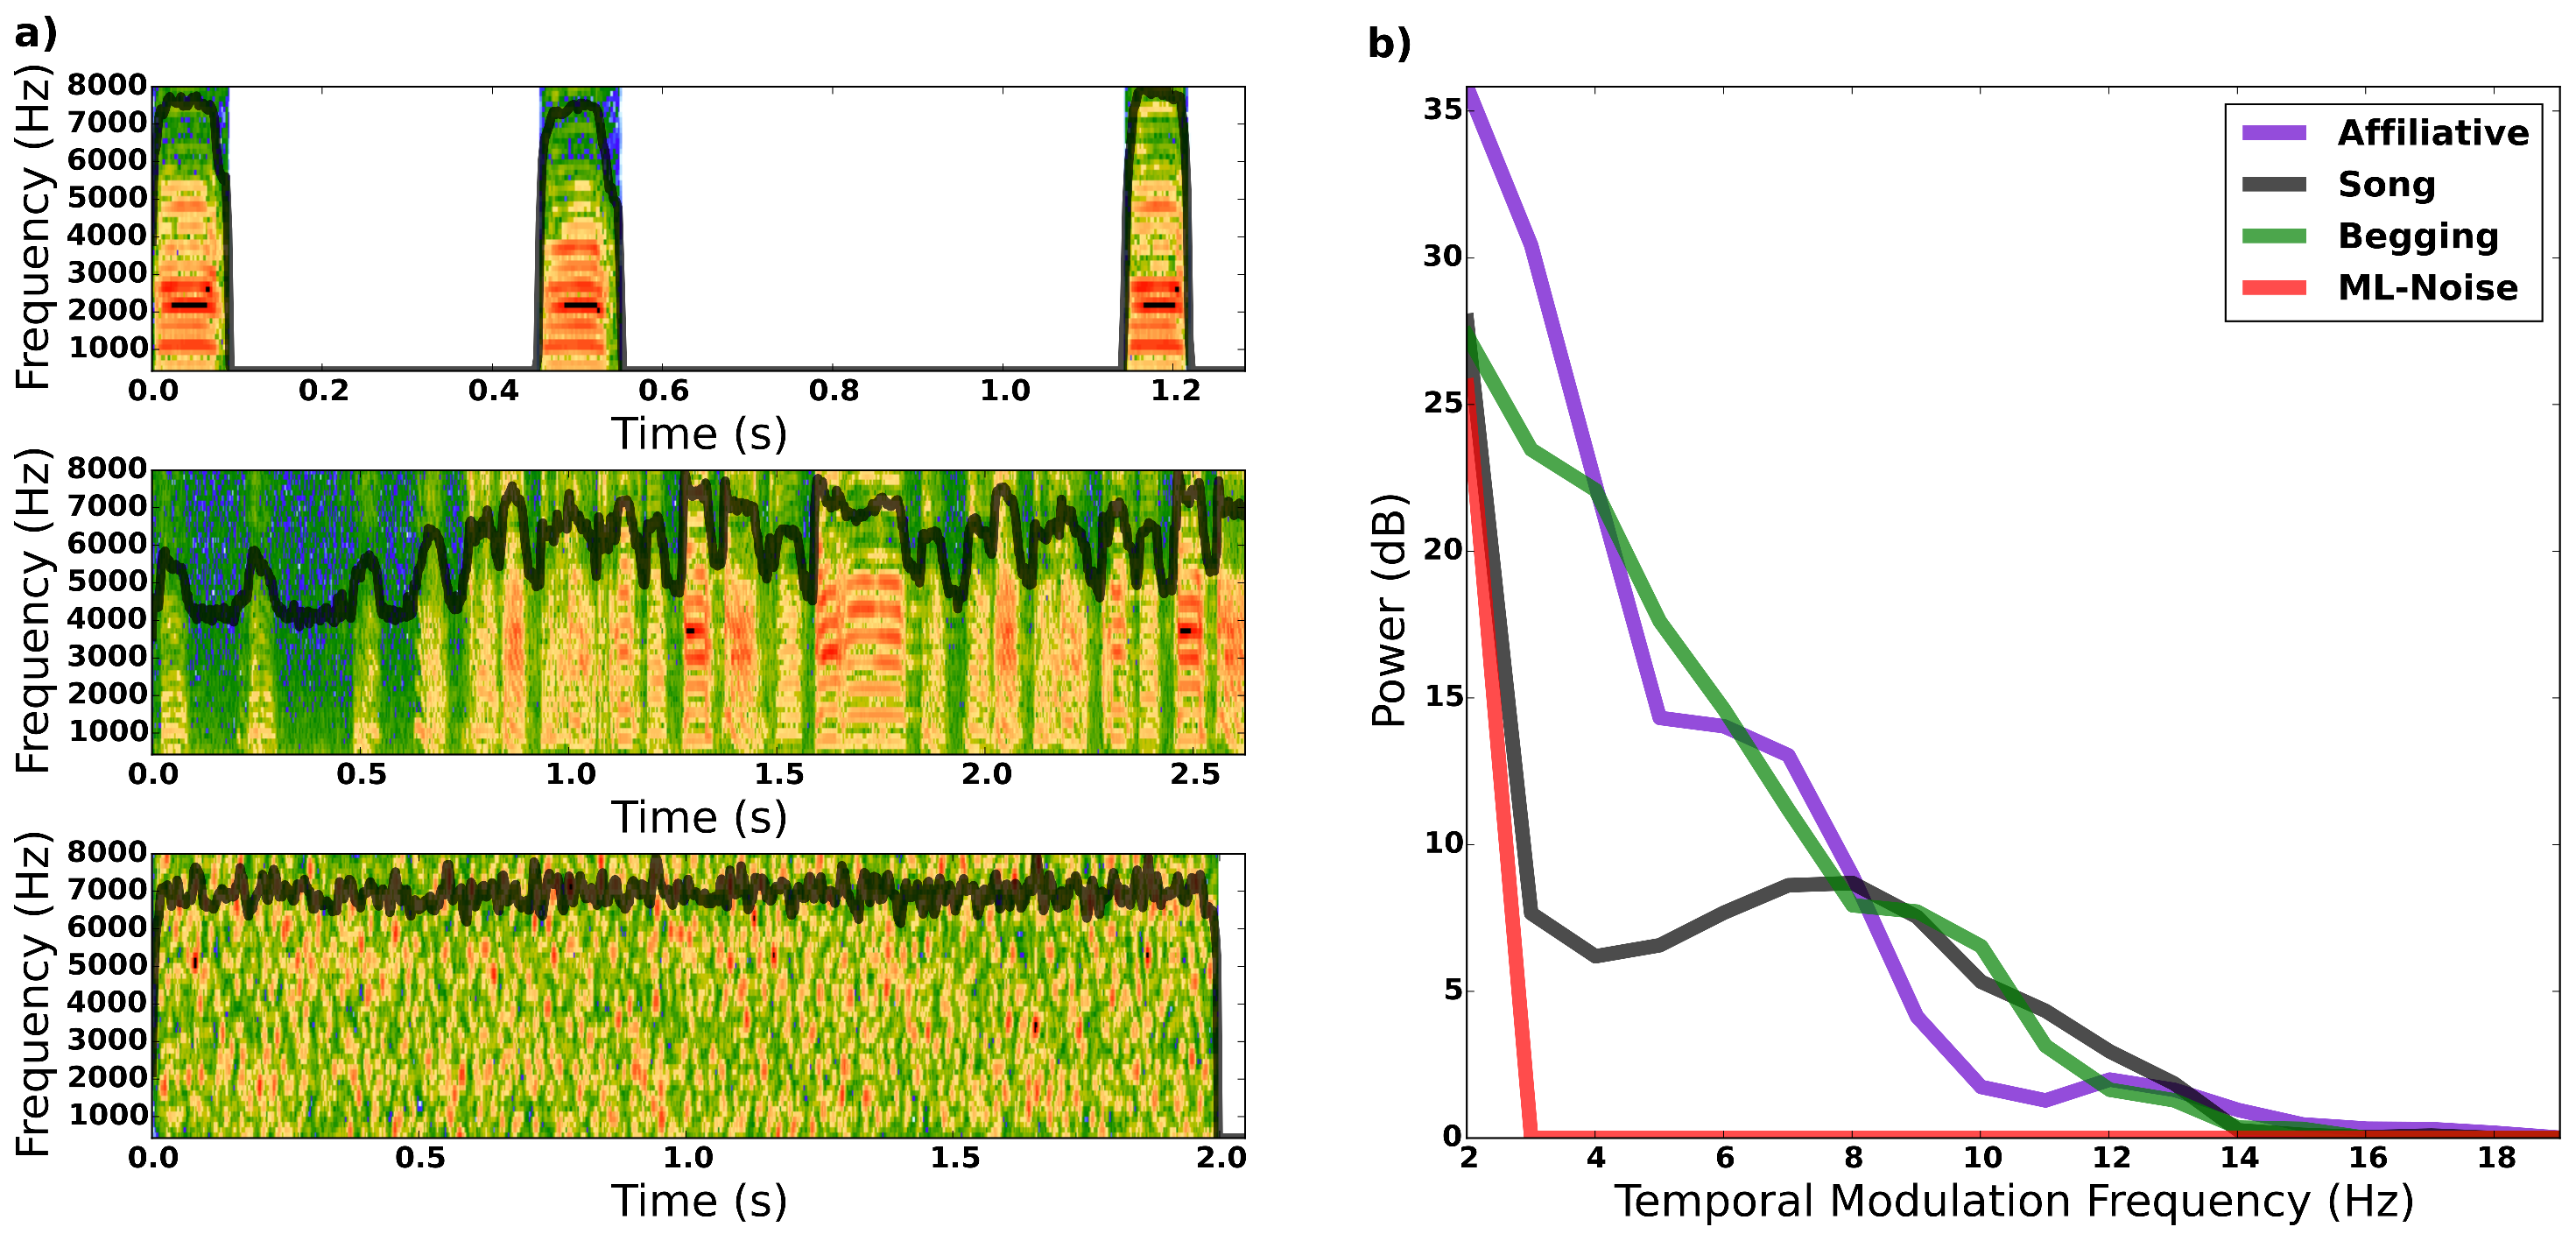
\includegraphics[scale=0.25]{figure_2_1.eps}
\end{figure}

\subsection{Linear Filter Encoders Predict LFP from Amplitude Envelope}

The temporal modulation of sound through the amplitude envelope is vital for speech perception, and has be successfully decoded from multi-electrode activity in human auditory cortex \cite{Pasley2012}. We showed that temporal modulations varied for different types of Zebra finch vocalizations, and that these modulations occur primarily in frequencies that are less than 30Hz. Our next goal was to investigate whether temporal modulations in this range were represented by neural activity in the Zebra finch auditory system. We trained linear filter encoder models to predict 5-30Hz LFP activity from the stimulus amplitude envelope (see Methods - Linear Encoder Fitting). In this setting, the linear filter encoder is equivalent to a ``temporal receptive field'', that maps the recent history for the stimulus amplitude envelope to the bandpassed voltage recorded as the LFP, similar to a STRF with only one frequency band \cite{Theunissen2000}.

    Figure 2 shows encoder predictions for an example song vocalization. Figure 2a shows the song vocalization as a spectrogram, along with the amplitude envelope. Figure 2b shows the multi-electrode LFP in black, and the linear encoder predictions in red.  For many electrodes, the LFP responded to high amplitude, temporally sharp, and pitch-salient syllable onsets with sharp downward deflections. The linear model matches some of the stronger downward deflections. Sharp signals such those downward deflections are high amplitude and high-bandwidth, and predicting such a signal requires a filter with a sharp onset response. Following the sharp negative deflections in the LFP, a complex series of lower amplitude, lower bandwidth, more oscillatory upward and downward deflections occur. The linear model can be seen to match some of this activity as well, implying, perhaps surprisingly, that it may be operate on two different time-frequency scales.

\begin{figure}
    \caption{\textbf{Linear Encoder Predictions for 5-30Hz LFP} We trained linear filter models to predict 5-30Hz LFP activity on a single electrode from the temporal envelope of Zebra finch vocalizations. \textbf{(a)} The spectrogram and temporal envelope (black) of a Zebra finch song. \textbf{(b)} The raw 5-30Hz LFP (black) and linear filter encoder prediction (red) for 16 electrodes simultaneously recorded during the song presentation. Electrodes are ordered rostral-caudal from top to bottom.}
    \centering
    \includegraphics[scale=0.25]{figure_2_2.eps}
\end{figure}

    We trained our linear encoders using a cross-validation approach (see Methods - Linear Encoder Fitting) and report the average cross-validation correlation coefficient between the model prediction on the holdout set and the actual LFP. Figure 3a shows performance for each electrode plotted by recording location. Electrodes rostral to the thalamorecipient region L2A had higher performances than electrodes caudal to L2A (ANOVA, F(1, 307)=16.4, p $<$ 0.01). Lateral distance from the midline was not a significant predictor of encoder performance (ANOVA, F(1, 307)=0.32, p=0.57). The Zebra finch auditory system is not a homogeneous structure, it is broken into regions with differing neuron densities and functional encoding properties. Figure 3b breaks down decoder performance by anatomical region. Encoder performance was significantly related to anatomical region (ANOVA, F(4, 317)=13.5, p $<$ 0.01). Performance was highest for regions in Field L, and lowest for region NCM.

\begin{figure}
    \caption{\textbf{Linear Encoder Performance for 5-30Hz LFP} \textbf{(a)} A map in anatomical coordinates of linear filter encoder performance, for electrodes across the dataset. Text annotations denote the anatomical region of the electrode. Electrodes on the left hemisphere were mirrored and superimposed with electrodes on the right hemisphere. \textbf{(b)} A boxplot of linear filter encoder performance by anatomical region. Performance was best in thalamorecipient region L2 and worst in secondary auditory region NCM.
}
    \centering
    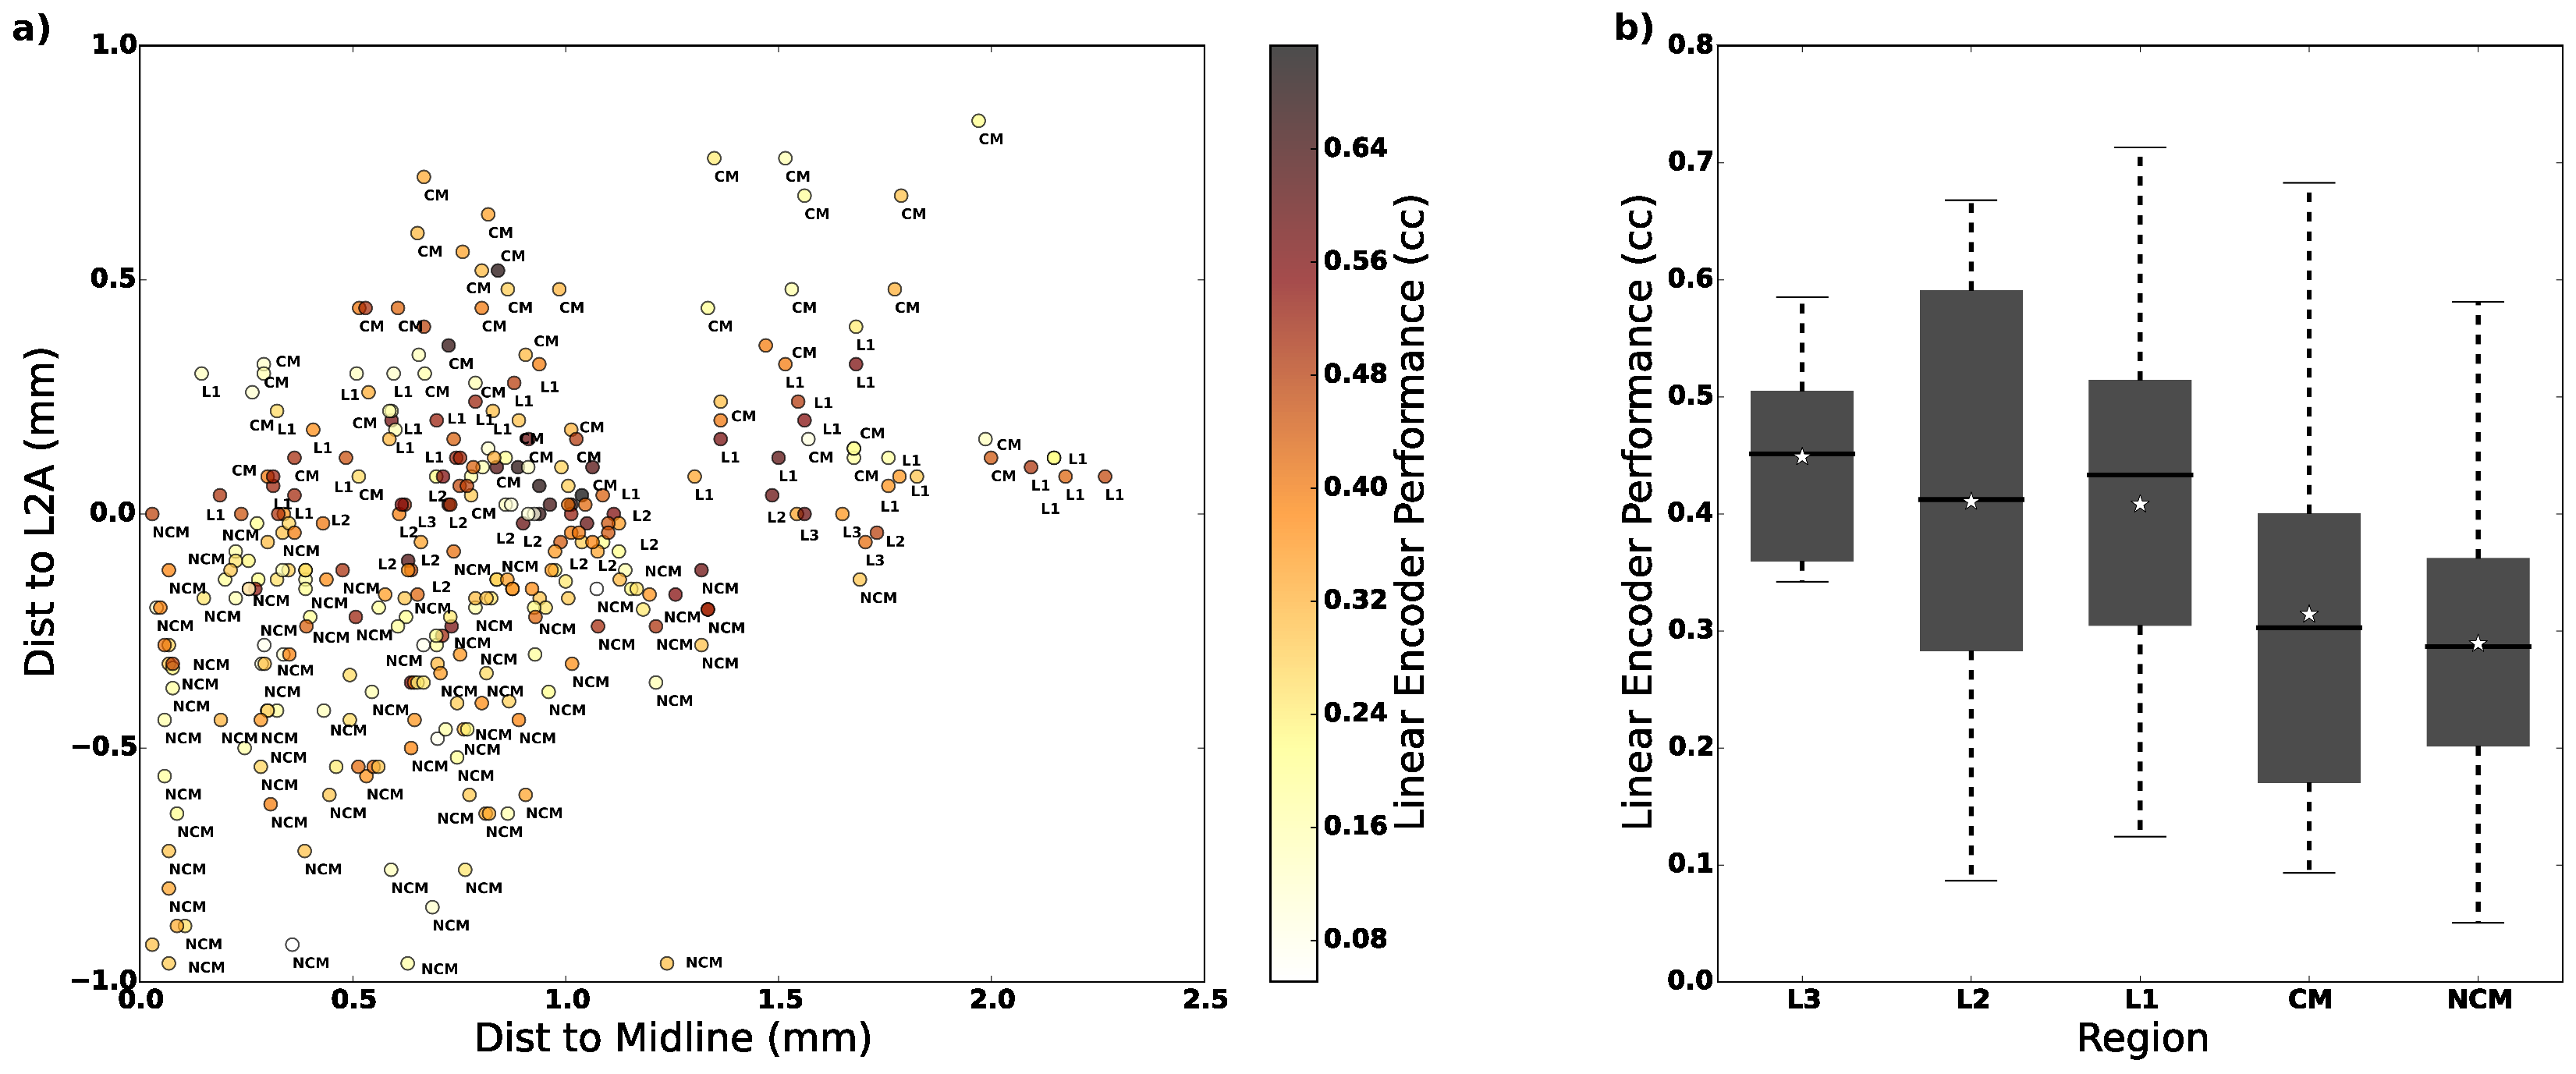
\includegraphics[scale=0.25]{figure_2_3.eps}
\end{figure}

\subsection{Two Oscillatory Subnetworks}

We observed in Figure 2 that the 5-30Hz LFP exhibited activity at two different time-frequency scales. The first timescale was a high amplitude, high bandwidth negative deflection that responded to syllable onsets, while the second was a lower bandwidth, lower amplitude, oscillating response. We analyzed the structure of the linear filters, plotted by region in Figure 4a. The filters had two major components, an initial sharp downward deflection, responsible for the onset response, and a slower oscillatory component that helped predict the resonant properties of the LFP. We quantified this oscillatory component by fitting it with a sine curve (see Methods - Linear Filter Frequency Fitting). In figure 4b we report the center frequencies of the oscillatory components. Surprisingly, the center frequencies fall into a bimodal distribution, one in the 10-15Hz band, and another sharply peaked around 20Hz. To quantify this, we pooled data across regions and fit a bimodal Gaussian Mixture Model to the data. The bimodal GMM outperformed a unimodal model (Likelihood Ratio Test, deviance=6.9, p $<$ 0.01), and best fit the data with two Gaussian distributions, one centered at 16Hz with a standard deviation of 3Hz, and another centered at 19Hz with a standard deviation of 4Hz. The analysis was re-run within each anatomical region wtih similar results. To summarize, our linear encoder analysis and investigation of the filters revealed two subpopulations in the auditory network that resonate at different frequencies, found in every anatomical region.

\begin{figure}
    \caption{\textbf{Distinct oscillatory subnetworks} We analyzed the linear filters of the encoder models to determine how they mapped the temporal envelope to the LFP. \textbf{(a)} Filters across anatomical regions had a common theme, a sharp response to amplitude envelope in the first 5ms, followed by a slower oscillatory component. \textbf{(b)} We quantified the oscillatory component for each filter by it’s best fit frequency, and here report the distribution of filter frequencies by anatomical region.
}
    \centering
    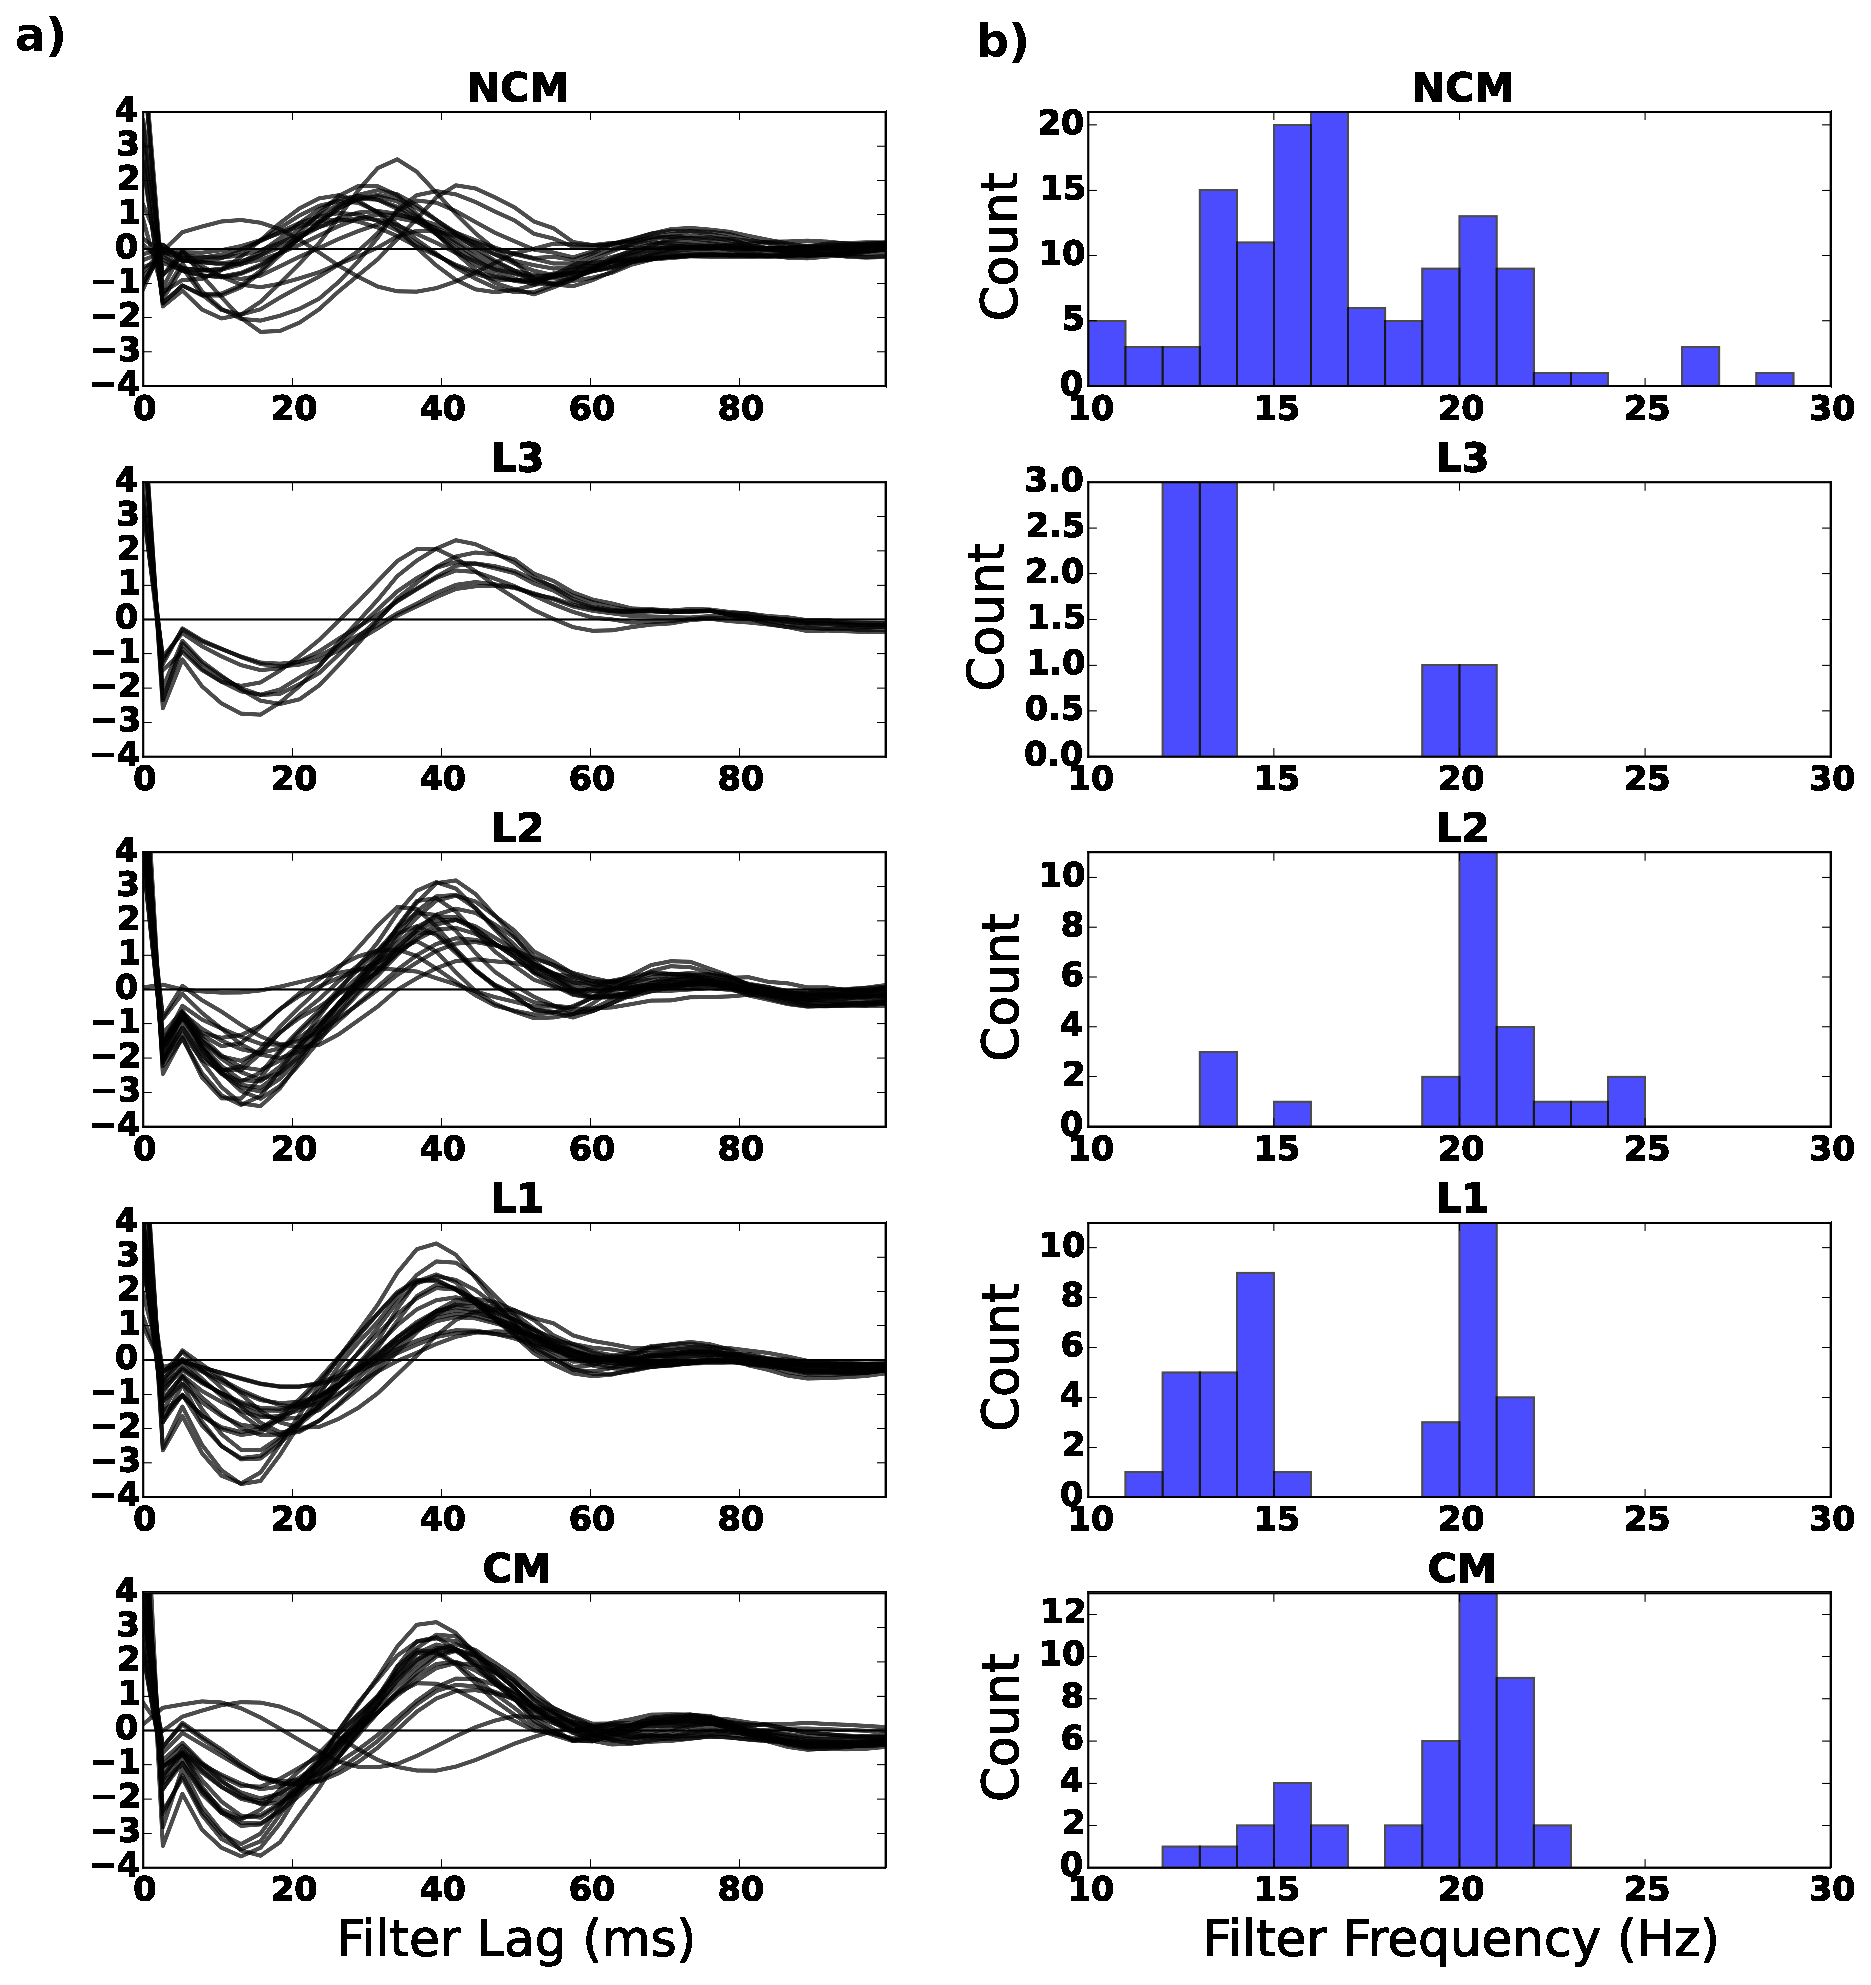
\includegraphics[scale=0.25]{figure_2_4.eps}
\end{figure}

\subsection{Recurrent Neural Networks Outperform Linear Models}

Although linear models performed very well for some regions, the predictions shown in Figure 2 are far from perfect. They miss many of the essential modulations that occur throughout the stimulus. In an attempt to fit the more nonlinear aspects between the temporal envelope and LFP, we trained recurrent neural networks (RNNs) to predict 5-30Hz activity from the stimulus amplitude envelope. A recurrent network is a trainable nonlinear filter, and we utilized the commonly used backpropagation through time algorithm to fit networks to the data (see Methods - Training Recurrent Neural Networks). Our RNN models outperform linear models on virtually every electrode, as shown in Figure 5, providing an average boost in correlation coefficient of 0.08 (paired t-test, t=-28.9, N=447, p$<$0.01).

\begin{figure}
    \caption{\textbf{Performance enhancements from using RNNs}  We fit recurrent neural networks to the data to predict the multi-electrode 0-30Hz LFP from the temporal envelope. We compared performance of linear encoders on the x-axis, with the performance of the RNN encoders on the y-axis. Nearly all the points lie above the unity line y=x, indicating that RNNs outperform linear models.
}
    \centering
    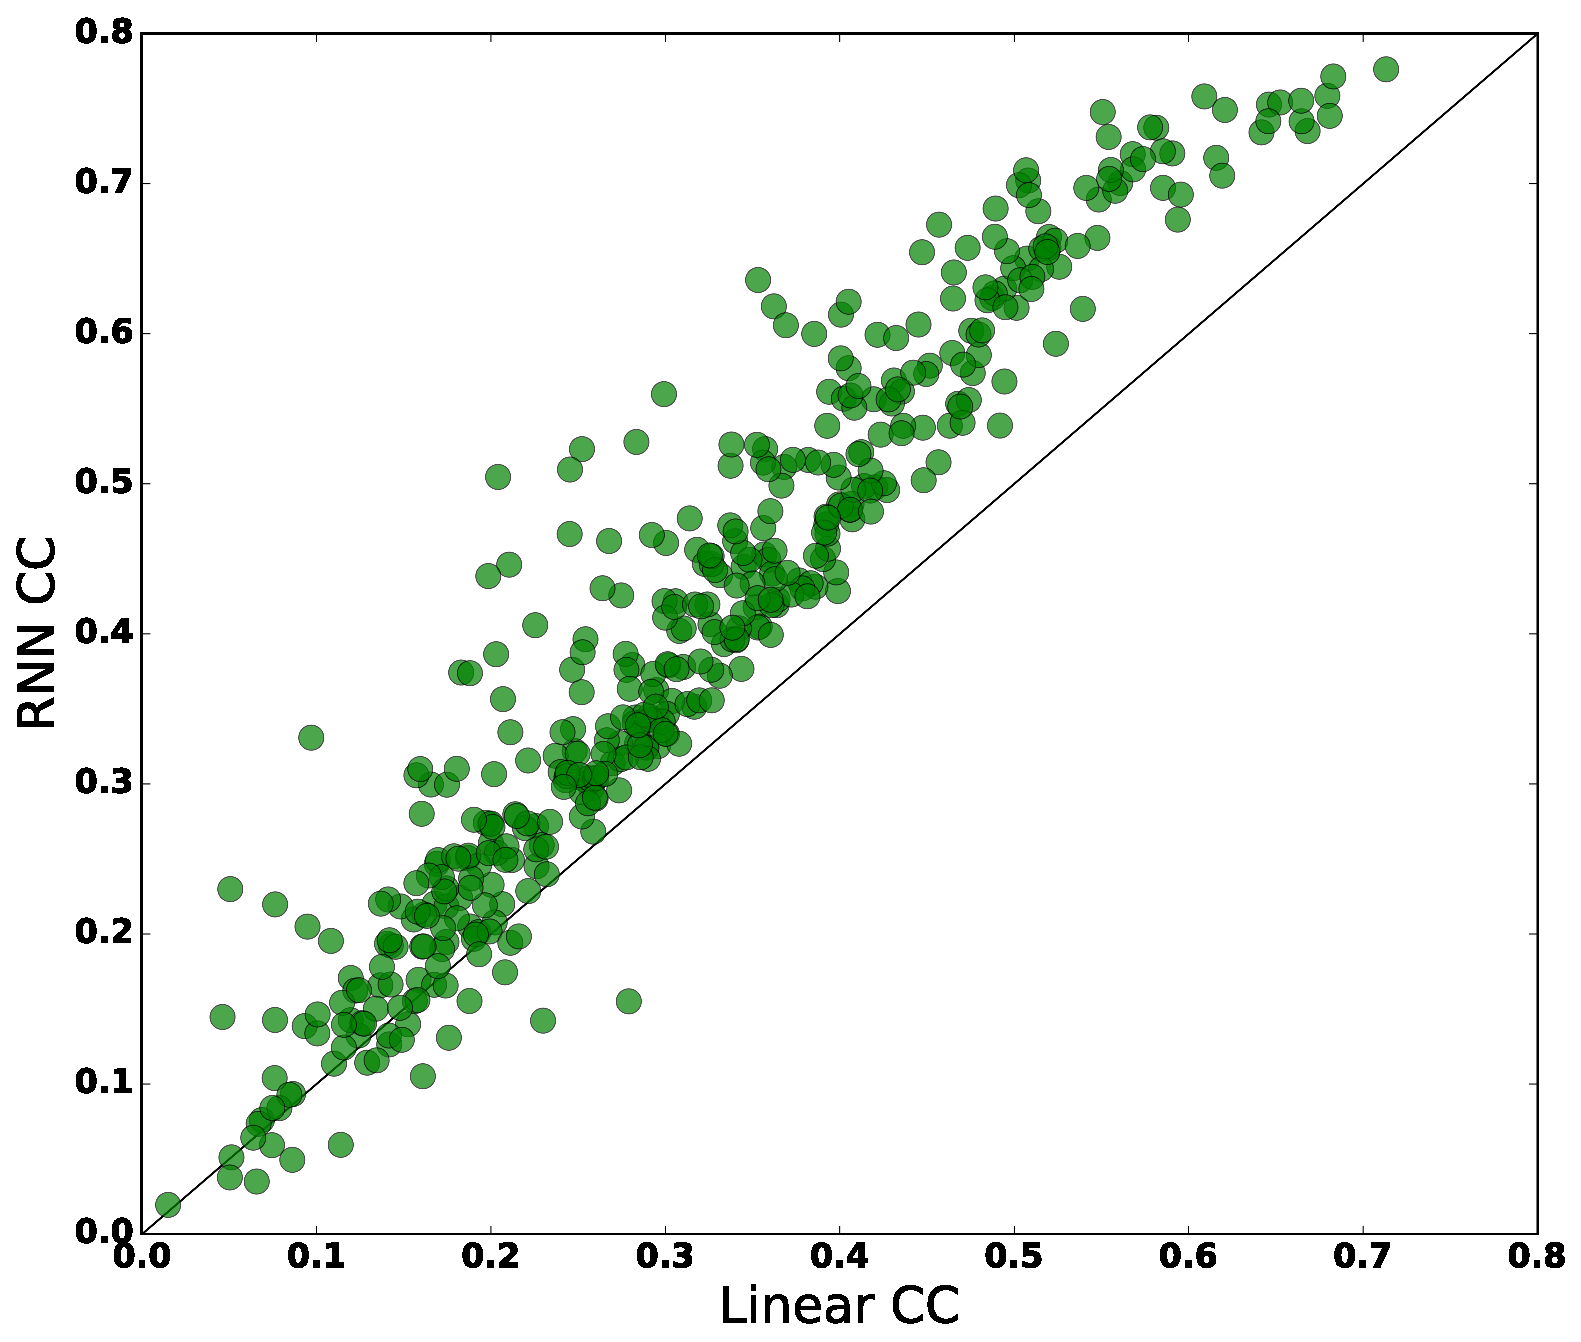
\includegraphics[scale=0.25]{figure_2_5.eps}
\end{figure}


\section{Discussion}

We first showed that the temporal modulations of the stimuli we utilized for the experiment fell in the 0-30Hz range, a range similar to the temporal modulations of human speech (\cite{Aiken2008}, \cite{Ding2016}). Notably, song stimuli had significant power in their temporal modulation spectra from 6-10Hz, which may be the ``natural'' frequencies of Zebra finch song. Begging calls, emitted by juveniles, occupied a similar range of frequencies as song, suggesting perhaps that Zebra finch brains are tuned to resonate at these frequencies, and juveniles take advantage of these natural frequencies to manipulate their parents.

Through linear modeling, we showed that the local field potential can be successfully predicted from the temporal envelope of our stimuli. The reverse direction, predicting the temporal envelope from multi-electrode LFP, was accomplished in human auditory cortex by \cite{Pasley2012}. We found encoder performance to be region-specific, with encoders performing the best in thalamorecipient regions, and the worst in secondary auditory region NCM. This could be due to differences in NCM activity for awake vs anesthetized subjects, or perhaps the function of neurons in NCM does not require the close following of the temporal envelope. There is evidence that neurons in NCM serve to ``de-noise'' stimuli and are more invariant to changes in background noise and amplitude (\cite{Schneider2013}, \cite{Moore2013}).

We were surprised to find two distinct oscillatory subnetworks in the Avian auditory system, consistent across every anatomical region. This complements the hypothesis of mammalian-like columnar microcircuitry suggested by \cite{Wang2010} and \cite{Calabrese2015}, who proposed the canonical microcircuit connects auditory thalamus to L2, then L2 to L1, then L1 to region CM. It’s possible that in order to communicate with each other, these regions must match oscillation frequencies in order to synchronize information transfer, a method of neural computation termed “communication by coherence” proposed by \cite{Fries2005}. It will be important in future work to study whether these oscillation frequencies change on a per-stimulus basis.

Finally, we showed that we could boost encoder performance by utilizing recurrent neural networks. In Figure 6 we show the predictions of the RNNs vs predictions of linear models. The RNN does a better job at fitting downward deflections that occur at stimulus onsets, but, disappointingly, does not do much better at capturing the non-onset oscillatory activity. We are actively engaged in work to improve both the performance and interpretability of these models. On the performance front, we had temporal limitations that prevented us from testing a fuller set of hyperparameters, and only utilized up to 100 neurons in the RNN. The LFP exhibits a significant amount spontaneous activity during silent periods, and there are RNN constraints that have been developed to ensure that population activity stays fixed at a baseline level throughout its lifetime \cite{Krueger2015}. Also, given that gamma oscillations originate from the interplay of excitatory and inhibitory neurons \cite{Buzsaki2012a}, we could constrain our network to be topologically organized and also enforce neurons to be either excitatory or inhibitory, as was done in \cite{Song2016}. Building multi-input, multi-output MIMO encoders with recurrent neural networks constrained to be more biologically plausible will allow us to ``peek in the black box'' of neural activity to further our understanding of neural dynamics.


\section{Methods}


Electrophysiological methods are fully described in \cite{Elie2015a} and \cite{Elie2015b} respectively and summarized here below. We then describe the methods used to preprocess the LFP, fit and analyze linear filter encoders to predict the 5-30Hz LFP, and train recurrent neural networks (RNNs) to predict the multi-variate 5-30Hz LFP waveforms. All animal procedures were approved by the Animal Care and Use Committee of the University of California Berkeley, and were in accordance with the NIH guidelines regarding the care and use of animals for experimental procedures.

\subsection{Animals}

The animal subjects studied were adult and juvenile zebra finches (Taeniopygia guttata) from the colonies of the Theunissen and Bentley labs (University of California, Berkeley, USA). The electrophysiology experiments were performed on four male and two female adults from the Theunissen lab colony. The acoustic recordings described in the next subsection involved twenty-three birds (eight adult males, seven adult females, four female chicks, four male chicks). Six adults (three males, three females) were borrowed from the Bentley lab.

The electrophysiology subjects were housed in unisex cages and allowed to interact freely with their cagemates. All subjects were in the same room and were could interact visually acoustically. The acoustic recordings were performed on pair-bonded adults housed in groups of 2-3 pairs. Chicks were housed with their parents and siblings.
    
\subsection{Zebra Finch Vocalization Types}

Zebra finches communicate using a repertoire of vocalizations that are dependent on behavioral context. Following \cite{Zann1996}, acoustic signatures and behavioral contexts were used to classify vocalizations into nine different categories. A detailed description of call categories can be found \cite{Elie2015a}. We provide here, a very succinct summary of that characterization for a subset of the calls analyzed here and used in the neurophysiological experiments.

Song is a multi-syllable vocalization emitted only by males. Songs are comprised of repeating motifs of syllables, and in the dataset, have a duration of 1424 +/- 983ms. Song in zebra finches are used in pair bonding and mating behavior. The repertoire contains monosyllabic affiliative calls used to maintain contact. Distance calls are loud, used when not in visual contact, and longer in duration (169 +/- 49ms) than Tet calls, emitted when in visual contact during hopping movements, with a duration of 81 +/- 16ms. Zebra finch also produce software calls used principally in the initial stages of pair bonding. Nest calls are soft monosyllabic vocalizations emitted by zebra finches looking for a nest or constructing a nest. With a duration of 95 +/- 75ms, they are similar to Tets.

Zebra finches emit two types of calls when they are acting out aggressively or being attacked. Wsst calls are noisy (broadband) and often long (503 +/- 499ms) calls emitted by a zebra finch when it is being aggressive. Distress calls are long (452 +/- 377ms), loud, and high-pitched vocalizations emitted by a zebra finch when escaping from an aggressive cage-mate. Both types of vocalizations can be mono or polysyllabic.

Two calls are emitted by juveniles only. Long tonal calls are the precursor to the adult distance calls; they are loud, long (durations of 184 +/- 63ms) and monosyllabic, emitted when the chick is separated from it’s siblings or parents. Begging calls are emitted when a juvenile zebra finch is begging for food from a parent, it is loud, long (duration of 382 +/- 289ms), and monosyllabic.

\subsection{Electrophysiology and Histology}

    Twenty-four hours before recording, the subject was deeply anaesthetized with isoflurane and injected topically with lidocaine in order to remove a patch of skin over the skull and cement a  head-holding fixture. On recording day, the subject was fasted for one hour, anaesthetized with urethane, head-fixed in a stereotaxic device, and two small rectangular openings were made over the auditory area of each hemisphere. An electrode array with two columns of eight tungsten electrodes was lowered into each hemisphere. Electrodes were coated in DiI powder so that their path through the tissue could be analyzed post-experiment. The electrodes ran rostral-caudal lengthwise in eight rows, with two columns that ran medial-lateral.

    During the experiment, the subject was placed in a soundproof chamber and electrode arrays were independently lowered. Probe stimuli were used to determine visually whether the areas were auditory. Once a reliable site was found, a stimulus protocol was played over speakers within the chamber (described in next subsection). When the stimulus protocol was complete, the electrodes were lowered deeper by at least 100 microns before playing the protocol again at the next site.
Once the recordings were finished, typically after 4-5 recording sites, the subject was killed with an overdose of isoflurane, the brain was removed and fixed with paraformaldehyde. Coronal slices of 20 microns were made with a cryostat and Nissl stained. The slices were examined under a microscope and the DiI tracts were used to determine electrode penetration through anatomical regions. Six auditory areas were differentiated: three regions of field L (L1, L2, L3), caudomedial and caudolateral mesopallium (CMM and CML), and caudomedial nidopallium (NCM).

\subsection{Stimulus Protocol}

    The vocalizations of ten individuals (three adult females, three adult males, four chicks) were used in the stimulus protocol. The vocalizations of four of the individuals (one male adult, one female adult, one male chick, one female chick) were played at each recording site, and three of each vocalization type were randomly selected from the other birds to be played. Each vocalization was played on average 10 times, randomly interleaved with other vocalizations. The protocol lasted an average of one hour. Monosyllabic vocalizations such as Distance and Tet calls were played with 3-4 different renditions in series with inter-syllable intervals chosen to match what was observed naturally.

\subsection{Sound Preprocessing}

Vocalizations used in the experiment were transformed into a spectrogram using custom python software. The spectrogram was computed by first applying a short-time Fourier transform (STFT) to the raw sound pressure waveform. The waveform was broken into overlapping segments of length 7ms, spaced apart by a sample interval of 1/381Hz, and segments were multiplied by a Gaussian window of length 6 standard deviations. The Fourier transform was then computed, the absolute value was taken, and squared, to produce the power spectrum corresponding to that segment. The log of the spectrogram was then taken.

To compute the stimulus amplitude envelope, the spectrogram was summed across frequencies at each time point. To compute the temporal modulation frequencies, each stimulus amplitude envelope was isolated, and a spectrogram was computed using a Gaussian window of length of 1s, with increments of 200ms. The windowed segments were averaged to produce the final temporal modulation spectrum.

\subsection{LFP Preprocessing}

The local field potential was recorded with a sample rate of 381 Hz. The LFP on each electrode was z-scored across time for the duration of a stimulus protocol. The LFP was then bandpassed with a pass band of 5-30Hz using a 5th order Butterworth filter implemented in Scipy.

\subsection{Linear Encoder Fitting}

We denote the value of the sound amplitude, for time $t$ during the stimulus protocol played at a site, as $x(t)$. We denote the value of the LFP on electrode $k$, at time $t$ during the stimulus protocol, as $u_k (t)$. Our goal was to build a linear filter model that predicted the LFP at a given time from the recent history of sound amplitude. To fit a filter using linear regression, we first created a feature vectors comprised of value of the stimulus amplitude envelope at time $t$, as well as $D$ lags into the past:

\begin{center}
$\textbf{x}_t = [x(t) \; ... \; x(t-D)]$
\end{center}

$D$ was chosen so that 500ms of recent stimulus history were taken into account. We then constructed a data matrix $X$ comprised of the feature vectors:

\begin{center}
$X = [\textbf{x}_1 \; ... \; \textbf{x}_{N}]^T$
\end{center}

where $N$ is the length of the stimulus protocol, with silent periods excluded. 500ms of zeros were inserted between stimuli so that they did not interfere with each other during fitting. $N$ was typically around $10^6$. The dependent variable was then the bandpassed LFP time series:

\begin{center}
$\textbf{y} = [u_k (1) \; ... \; u_k (N)]$
\end{center}

A linear filter was found that optimally mapped the stimulus history vector to the bandpassed LFP by minimizing the sum of squares error in prediction:

\begin{center}
$L(X, \textbf{y}, \textbf{w}) = || (X\textbf{w} + b) - \textbf{y} ||^2$ 
\end{center}

We utilized Ridge regression with scikits.learn to do this regularization. Ridge regression computes the optimal linear filter \textbf{w} as:

\begin{center}
$ \textbf{w} = (X^T X - \lambda I)^{-1} \; X^T \textbf{y}$
\end{center}

the value $\lambda$ is a user-defined hyperparameter, high values of $\lambda$ force weights towards zero. 

The value of the hyperparameter $\lambda$ was fixed to 1.0, because observations from several electrodes demonstrated very similar results for many different values of $\lambda$. 10-fold cross validation was used to compute the cross-validated correlation coefficient. The N samples were split into 10 partitions. For each partition, the rest of the data was trained on, and the correlation coefficient was computed between the prediction on the partition and the actual time series. We report here the correlation coefficients averaged across the ten partitions of data.

\subsection{Linear Filter Frequency Fitting}

To determine the frequency of the oscillatory component of a linear filter, we first isolated the filter between 5ms and 80ms lags, and normalized it by dividing by the absolute maximum. We then fit a sine curve $sin(2\pi t f + \phi)$, where $f$ was the center frequency and $\phi$ was a phase offset, both free variables. We utilized the Scipy curvefit function to fit the curves.

\subsection{Training Recurrent Neural Networks}

We utilized a recurrent neural network (RNN) architecture to predict multi-electrode LFP activity in the 5-30Hz range from the time-varying stimulus amplitude envelope x(t). Let $\textbf{u}(t)$ be the time-varying multi-electrode LFP:

\begin{center}
$\textbf{u}(t) = [u_1 (t) \; ... \; u_M (t)]$
\end{center}

where $M$ is the number of electrodes. Our recurrent neural network architecture uses recurrently connected hidden units to nonlinearly filter the time-varying input $x(t)$. A weighted combination of hidden unit activity is used to make a prediction of the multivariate LFP at time $t$. Let $\textbf{z}(t)$ be a vector of hidden unit states at time $t$ for a recurrent network of $D$ neurons:

\begin{center}
$\textbf{z}(t) = [z_1 (t) \; ... \; z_D (t)]$
\end{center}

The dynamics of our recurrent networks are given by:

\begin{center}
$ \textbf{z}(t+1) = \sigma \left( R \textbf{z}(t)  + W x(t) + \textbf{b} \right)$
\end{center}

where $\sigma$ is the logistic sigmoid function, $R$ is a $D$x$D$ matrix of recurrent weights, $W$ is a $D$x$1$ matrix of input weights, and $\textbf{b}$ is a vector of $D$ bias weights. The prediction of the LFP at time $t$ is given as a weighted combination of hidden states:

\begin{center}
$\hat{\textbf{u}}(t) = W_{out} \textbf{z}(t)$
\end{center}

where $W_{out}$ is a $M$x$D$ matrix of output weights.

    We used a truncated backpropagation through time algorithm (BPTT) \cite{Werbos1990} to simultaneously fit $R$, $W$, $b$, and $W_{out}$. The data was broken into segments of length $\tau_{mem}$=50 time points. The cost function that was minimized for each segment was specified as:

\begin{center}
$L(x(t), \textbf{u}(t), R, W, \textbf{b}, W_{out}) = \sum _{\tau = \tau_i} ^{\tau_f} || \hat{\textbf{u}}(\tau) - \textbf{u}(\tau) ||^2 + \lambda_2 \sum _{ij} R_{ij}^2 + \lambda_1 \sum_{ij} |R_{ij}|$
\end{center}

where $\lambda_1$ and $\lambda_2$ are hyperparameters for L1 and L2 regularization, and $\tau_i$ and $\tau_f$ are the start and end times of the segment, respectively. It should be noted that the cost function requires the value of $\textbf{z}(\tau_i - 1)$ to be specified. We trained segments sequentially, so that the hidden state corresponding to the end of the previously segment was used as the initial state for the next segment. This provided the network the opportunity to extend memory well past the segment size $\tau_{mem}$.






















